\chapter{Tecniche basate sul grafo}
\lstset{basicstyle=\small\ttfamily,keywordstyle=\color{black}\bfseries,commentstyle=\color{darkgray},stringstyle=\color{black},showstringspaces=true}
In questo capitolo verrano presentate le tecniche di spam detection presenti in letteratura, denominate \textit{linked base}, che si avvalgono cioè del grafo del web  derivato dalla fase di crawling, che si ricava dai collegamenti ipertesuali tra le pagine. Il web può essere rappresentato come un grafo orientato \textit{G = (V,E)} dove \textit{V} è l'insieme dei nodi del grafo e rappresenta le pagine web, ed \textit{E} è l'insieme degli archi  orientati tra i nodi e rappresenta l'insieme dei link orientati tra le pagine; assumendo che ci siano due pagine web \(a_p\) e \(b_p\) queste saranno rappresentate da due nodi del grafo \(a\) e \(b\); se esiste un collegamento ipertestuale  dalla pagina \(a_p\) alla pagina \(b_p\) allora vi sarà un arco diretto dal nodo \(a\) al nodo \(b\). 

Ogni pagina ha:
\begin{itemize}
 \item  link in uscita (\textit{outlink}) ovvero i link presenti nella pagina che referenziano altre pagine web;
 \item  link in entrata (\textit{inlink}) ovvero tutti i riferimenti della pagina fatti da altre pagine.
\end{itemize}

Il grafo del web può essere astratto e rappresentato da una matrice di transizione cosi formata:
\begin{equation}
T(p,q)=\left \{
\begin{array}{cc}
0 & if(p,q) \not\in E\\
1/\omega(p) & if(p,q) \in E
\end{array}
\right .
\end{equation}
dove \(q\) e \(p\) sono delle pagine web appartenenti al grafo e \(\omega(p)\) è il grado di link in uscita della pagina \(p\). 
Possiamo anche definire la matrice di transizione inversa U:
\begin{equation}
U(p,q)=\left \{
\begin{array}{cc}
0 & if(q,p) \not\in E\\
1/l(p) & if(q,p) \in E
\end{array}
\right .
\end{equation}
dove \(l(p)\) è il grado di link in ingresso della pagina \(p\). Bisogna notare che \(U \not = T^T\), ovvero la matrice di transizione inversa \(U\) non è uguale alla matrice di transizione trasposta.
\section{Metodi classici per identificare lo spam web usando il grafo}
Uno dei primi metodi adottati di spam detection che utilizza il grafo del web è \textit{Trustrank} \cite{Gyongyi:2004:CWS:1316689.1316740}. \textit{Trustrank} applica a un insieme di pagine di partenza \(S\) (detto anche seedset) una funzione \textit{Oracle} per classificare il seedset in due sottoinsiemi, pagine non spam \(S^+\) e pagine spam \(S^-\); tale classificazione è effettuata manualmente da esperti. Per determinare le pagine non spam senza invocare la funzione \textit{Oracle} su tutto il grafo derivato dalla fase di crawling, viene fatta un'assunzione empirica chiamata \textit{isolazione approssimata dell'insieme delle pagine buone}, la quale afferma che le pagine non spam raramente punteranno a delle pagine spam. Razionale di tale assunzione è che gli sviluppatori di pagine web non spam non hanno interesse nel linkare pagine spam (a meno che  tramite l'uso di tecniche come l'\textit{honeypot} vengano ``ingannati''). Quindi fissato un numero limitato di chiamate della funzione \textit{Oracle} sul 
seedset di partenza e sfruttando l'assunzione fatta precedentemente viene definita una funzione, denominata \textit{funzione di verità ignorante \(T_0\)}, per ogni pagina pagina \(p\) del grafo:
\begin{equation}
T_0(p)=\left\{
\begin{array}{ccc}
O(p) & if & p\in S \\
1/2 & altrimenti
\end{array}
\right .
\end{equation}
dove la funzione \(O\) è la funzione \textit{Oracle}. Presupponendo che le pagine non spam puntino ad altre pagine non spam viene assegnato il valore 1 a tutte le pagine che possono essere raggiunte da una pagina in \(S^+\) in \(M\) step. La funzione di verità \(T_M\) è definita come:
\begin{equation}
T_M(p)=\left\{
\begin{array}{ccccc}
O(p) & if & p\in S \\
1 & if & p \not\in S & and & \exists q\in S^+:q\rightarrow_M p \\
1/2 & altrimenti
\end{array}
\right .
\end{equation}
Il percorso  dalla pagina \(q\) a \(p\) nell'equazione non comprende pagine spam incluse nell'insieme \(S^-\).
\begin{figure}
\centering
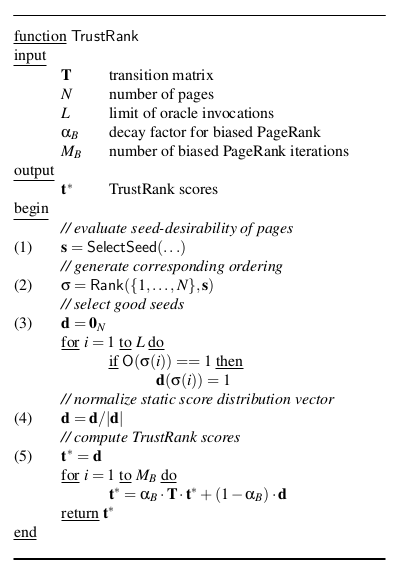
\includegraphics[width=8cm]{immagini/trustrank/trustrank}
\caption{Algoritmo di trustrank}
\label{fig:trustrank1}
\end{figure}
Limite della funzione di verità \(T_M\) è che si basa su un'euristica, quindi non esiste la sicurezza che le pagine raggiungibili da pagine non spam siano effettivamente della pagine non spam; tale sicurezza si riduce quanto più lontana dal seedset \(S^+\) è una pagina \(p\). Per non incorrere in tale errore si può ridurre il valore della funzione di verità in maniera proporzionale alla distanza dal seedset \(S^+\).

In figura \ref{fig:trustrank1} è illustrato lo pseudo-codice dell'algoritmo di \textit{Trustrank}; sarà descritto in dettaglio come funziona. 

I valori di input dell'algoritmo sono:
\begin{itemize}
 \item il grafo descritto dalla matrice di transizione \(T\);
 \item il numero di pagine \(N\);
 \item i parametri di controllo dell'esecuzione: \(L\) è il numero di chiamate della funzione \(Oracle\), \(\alpha_b\) è il fattore di decadimento per il calcolo di \textit{PageRank} ed infine \(M_b\) è il numero di iterazioni per il calcolo di \textit{PageRank}.
\end{itemize}

Al primo passo viene invocata la funzione \textit{SelectSeed()} che calcola l'insieme delle pagine con un relativo punteggio di pertinenza da includere nel seedset di partenza. Gli autori consigliano due metodi per implementare questa funzione : 
\begin{itemize}
 \item il primo metodo, chiamato \textit{Inverse PageRank}, attribuisce una preferenza alle pagine dalle quali si possono raggiungere molte altre pagine,  applicando l'algoritmo di PageRank sul grafo trasposto;
\item il secondo metodo, detto \textit{High PageRank}, assegna un alto valore di pertinenza a pagine che hanno un alto valore di pagerank.
\end{itemize}

Nell'istruzione (2) della figura \ref{fig:trustrank1} la funzione \(Rank(x,s)\) ordina gli elementi di \(x\) in modo decrescente sulla base dello score di \(s\). 

Nel punto (3) della figura \ref{fig:trustrank1} invoca la funzione \textit{Oracle} su \(L\) pagine, impostando a 1 i valori del vettore \(d\) che rappresenta l'insieme delle pagine del seedset.

Nel punto (4), ai valori del vettore \(d\), viene applicata una normalizzazione in modo tale che la somma faccia 1. 

Infine al punto (5) viene calcolato \textit{Trustrank} usando \textit{Pagerank} dove il vettore di teletrasporto è rimpiazzato dal vettore \(d\). Dall'algoritmo si nota che \textit{Trustrank} è una versione personalizzata di \textit{Pagerank} dove il vettore di teletrasporto è il seedset \(S^+\) calcolato al punto 3 e 4. L'obbiettivo è quindi assegnare un valore di verità alto alle pagine non spam e basso per le pagine spam.


Un altro algoritmo progettato per identificare lo spam usando come input il grafo delle pagine web è \textit{Anti-Trust Rank} \cite{Krishnan06webspam}. Partendo dalla stessa intuizione dell'isolamento approssimato ovvero che pagine non spam molto raramente puntino a pagine malevoli, \textit{Anti-trust rank}  popola un seedset formato da pagine spam e propaga la funzione Antitrust (corrispondente alla funzione di verità di Trustrank) sul grafo trasposto con l’obbiettivo di rilevare le pagine spam, che potranno quindi essere filtrate da un motore di ricerca. Più precisamente, a differenza di quanto avviene in \textit{Trustrank} dove la funzione \textit{Trust} è propagata dal seedset composto da pagine non spam lungo tutto il grafo, in \textit{Anti-Trust Rank} la funzione \textit{Anti Trust} è propagata nella direzione inversa ai link in entrata ad ogni pagina del grafo, partendo da un insieme di pagine del seedset composto da pagine spam. L'obbiettivo è assegnare un rank maggiore alle pagine spam e 
successivamente eliminarle dalle ricerche impostando un valore soglia tramite il quale escluderle oppure restituendo le \(n\) pagine che hanno valore di \textit{Anti-Trust Rank} più alto.
 
\textit{Trustrank} e \textit{Anti-Trust rank} sono ottimi algoritmi per identificare lo spam ma hanno il problema relativo alla dimensione dell’insieme  seedset, in quanto tale seedset potrebbe non essere sufficientemente rappresentativo per campionare tutti gli argomenti del web. Per tentare di risolvere questo problema è stato implementato un metodo \cite{Wu:2006:TTU:1135777.1135792}  che fa uso degli argomenti delle pagine come segnale di ingresso;  invece di usare un singolo valore di \textit{trustrank} per un nodo, vengono estrapolati per ogni pagina gli argomenti contenuti. L'algoritmo partiziona il seedset sulla base dei vari argomenti che esso contiene e usa ognuna di queste partizioni come seedset di partenza per calcolare il valore di \textit{trustrank} per ogni pagina.

 In letteratura viene descritto un metodo di spam detection  \cite{Caverlee:2007:CWS:1281100.1281124} \textit{linked base} che è difficilmente manipolabile tramite tecniche come \textit{honeypot}, a differenza dei precedenti metodi illustrati in questo capitolo . Infatti tale metodo separa la credibilità di una pagina dalla credibilità del link per quella pagina. La credibilità viene definita in termini di credibilità \textit{k-scope}. Sia una funzione \(C\) una funzione di credibilità che istantaneamente valuta la qualità di un link di un pagina \(p\) al tempo \(t\), per valori di \(C(p,t)=0\) la funzione indica che \(p\) non è credibile mentre per  \(C(p,t)=1\) la funzione indica che \(p\) è credibile. Sia un percorso in un grafo diretto \(G\) dalla pagina \(p\) alla pagina \(q\) la sequenza di nodi: \(path(p,q)=(n_0,n_1,...,n_j)\) dove \(p=n_0, q=n_j\) tale che esista un arco diretto tra nodi successivi nel percorso \(n_i,n_{i+1}\in L\) per \(0\leq i \leq j-1\), si definisce \textit{bad path} quel 
percorso  in un grafo  diretto \(G\)  dalla pagina \(p\) alla pagina \(q\) se la pagina di destinazione è una pagina spam \(q\in P_b\) (dove \(P_b\) è l'insieme delle pagine spam) e nessuna altra pagina nel percorso è una pagina spam ovvero \(path(p,q)=(n_0,n_1,...,n_j)\) e \(q\in P_b\) e \(n_i\not\in P_b (0\leq i\leq j-1)\). La probabilità che una camminata casuale passi attraverso un percorso di lunghezza \(k\) da una pagina \(p\) è denotata con \(Pr(path_k(p))\) ed è determinata con i pesi degli archi per ogni hop nel percorso:
\begin{equation}
 PR(path_k(p))=\prod_{i=0}^{k-1}w(n,n_{i+1})
\end{equation}
Quindi la credibilità \textit{k-scope} di una pagina  è definita in termini di probabilità che una camminata casuale eviti le pagine spam dopo aver superato \(k\) hop dalla pagina di origine. La credibilità \textit{k-scope} di una pagina \(p\) al tempo \(t\), denotata con \(C_k(p,t)\), è definita come segue:
\begin{equation}
 C_k(p,t)=1-\sum_{l=1}^k\left (\sum_{path_l(p)\in BPath_l(p)}Pr(path_l(p))\right )
\end{equation}
Dove \(BPath_l(p)\) è l'insieme di tutti i \textit{bad path} di lunghezza \(l\) che hanno origine dalla pagina \(p\). Appare chiaro che nel caso in cui \(p\in P_b\) allora la credibilità \textit{k-scope} è uguale a \(C_k(p,t)=0\). Se non ci siano pagine spam all'interno di \(k\) hop  allora la pagina \(p\) è credibile con un valore \(C_k(p,t)=1\). Il metodo descritto presenta tuttavia due criticità:
\begin{itemize}
 \item è difficile costruire un grafo che rappresenti interamente tutto il web;
 \item non si conoscono tutti i nodi spam.
\end{itemize}
 Per risolvere tali criticità è stato introdotto il concetto di \textit{tunable k-scope},  il quale modifica il calcolo della credibilità k-scope includendo un fattore di penalità di credibilità. Gli obbiettivi sono approssimare al meglio la credibilità \textit{k-scope} sotto limiti reali e capire come parametri differenti protrebbero influire sulla qualità delle varie funzioni usate. \\Sia \(G=(P,L)\) un grafo diretto, \(k\) il raggio massimo di camminata e \(\gamma(p)\) il fattore di penalità di credibilità di una pagina \(p\in P\) dove \(0\leq \gamma(p)\leq 1\), si definisce la credibilità \textit{tunable k-scope} di una pagina \(p\), denotata con \(C_k(p)\), in due fasi, quando \(p \not \in P_b\):
\begin{equation} 
C_k(p)=\left ( 1 -\sum_{l=1}^k \left ( \sum_{path_l(p)\in BPath_l(p)} Pr(path_l(p)) \right ) \right ) \cdot\gamma(p)
\end{equation}
e quando \(p\in P_b\) allora: \(C_k(p)=0\).

Oltre a tale metodo per definire la credibilità di un link, gli autori in \cite{Caverlee:2007:CWS:1281100.1281124} propongono un algoritmo di ranking  basato sulla credibilità denominato \textit{CredibleRank}. \textit{CredibleRank} definisce che la qualità di una pagina è determinata da due criteri: la qualità delle pagine che puntano ad essa e la credibilità di ogni pagina puntata. Definendo con \(In(p)\) l'insieme di pagine che puntano a \(p\), si calcola \textit{CredibleRank} \(r_c(p)\) per una pagina \(p\):
\begin{equation}
r_c(p)=\sum_{q\in In(p)}C(q)\cdot r_c(q)\cdot w(q,p)
\end{equation}
Dalla formula si evince che il valore di \textit{CredibleRank} di una pagina \(p\) è determinato dalla qualità delle pagine che la puntano \(r_c(q)\) e dalla credibilità dei link \(C(q)\) delle pagine che la puntano cosi come la forza del link \(w(q,p)\).

Altri metodi di spam detection usano dei sottografi ricavati a partire dal grafo ottenuto dalla fase di crawling per rilevare lo spam. Ad esempio in \cite{Leon-Suematsu:2011:WSD:2052138.2052339} lo spam viene neutralizzato tramite l'identificazione di sottografi composti da pagine spam e i sottografi composti da pagine non spam.  
\begin{figure}
\centering
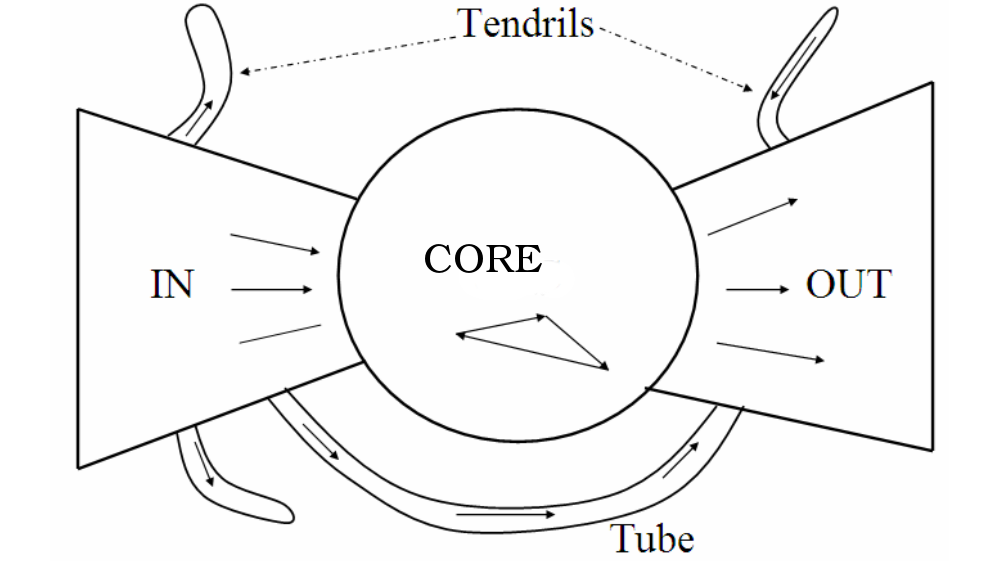
\includegraphics[height=7cm]{immagini/sub/sub}
\caption{Struttura bow-tie.}
\label{fig:sub}
\end{figure}
Il metodo elabora il grafo del web a due livelli di granularità, uno a livello di pagine web  e l'altro a livello di host. 

Il primo passo consiste nel rilevare gli host e le pagine spam partizionando il grafo in sottografi densi e calcolando delle feature per ogni sottografo sia sulla base degli URL (statistiche basate sulla lunghezza, statistiche basate sulla posizione della pagina rispetto all'homepage e statistiche basate sulla lunghezza del nome dell'host) e feature basate sul grafo. In particolare per rilevare i sottografi spam si analizza la struttura \textit{bow-tie} del grafo del web che si ottiene identificando le componenti fortemente connesse. In figura \ref{fig:sub} si nota che la struttura \textit{bow-tie} è composta da 5 elementi:
\begin{itemize}
 \item il \textit{Core} che è la componente fortemente connessa che contiene la maggior parte di siti non spam che sono facilmente accessibili agli utenti;
 \item la componente \textit{IN} è formata da pagine che puntano al \textit{Core};
 \item la componente \textit{OUT} è formata da pagine che sono puntate dal \textit{Core};
 \item le componenti \textit{Tendrils} che sono connesse alle componenti \textit{IN} o \textit{OUT} e la componente \textit{Tube}.
\end{itemize}
Quindi le pagine più facilmente accessibili sono quelle che si trovano all'interno della componente \textit{OUT}. Alcuni studi asseriscono che la presenza di dense componenti fortemente connesse vicino al \textit{Core} del grafo del web sia un indicatore potenziale di spam quindi per identificare i sottografi composti da pagine spam occorre analizzare ed individuare componenti fortemente connesse lungo \textit{In}, \textit{Out}, \textit{tendrils} e \textit{tube}.

Il secondo passo consiste nel ricondurre  a livello di host i valori di spam sia a livello di pagine che di host.

Successivamente vengono identificate le strutture fortemente connesse all'interno del \textit{Core} del grafo del web per rilevare gli host non-spam. L'identificazione dei sottografi non spam avviene all'interno della sezione \textit{Core} del grafo del web. Si definisce \textit{k-core} il massimo sottografo dove ogni nodo è connesso ad almeno \textit{k} altri nodi nel sottografo e il valore di \textit{coreness} di un nodo il massimo \textit{k} tale che il nodo venga classificato nel sottografo con il medesimo \textit{k-core}. Host molto importanti, ovvero quelli che hanno molti \textit{inlink}, sono connessi a altri host altamente connessi formando sottografi robusti con alta \textit{coreness}, mentre gli host spam hanno una bassa \textit{coreness}. Quindi impostando un certo valore di \textit{coreness} si possono identificare i sottografi con una certa robustezza e identificare soli i sottografi non spam.

Infine per aumentare il numero di host spam e non spam vengono propagati simultaneamente \textit{trustrank} e \textit{anti-trust rank}, dagli host che siamo sicuri siano non spam e spam agli host vicini in modo da valorizzare gli host non spam e penalizzare quelli di spam.

Un altro metodo per rilevare lo spam utilizza un classificatore automatico che combina un insieme di feature basate su link e contenuto \cite{Castillo:2007:KYN:1277741.1277814}. Considerando che i link tra le pagine non sono disposti in modo casuale ovvero pagine simili tendono a linkarsi tra di loro più frequentemente di pagine diverse, si può sfruttare tale meccanismo per rilevare le pagine spam che tendono a raggrupparsi in cluster. Infatti le pagine spam per aumentare il rank basato sui link utilizzano le link farm che costituiscono dei cluster all'interno del grafo. Da queste considerazioni gli autori assumono che gli host ben collegati tra di loro appartengano molto probabilmente alla stessa classe: spam o non spam.

\section{Metodi per identificare link farm}
Per riconoscere una spam farm (o link farm) si parte dal presupposto che i nodi della spam farm hanno dei link uscenti verso delle pagine target \textit{t} per aumentarne il rank. In \cite{Gyongyi:2006:LSD:1182635.1164166} per identificare le spam farm viene introdotta una misura denominata \textit{spam mass}, che valuta, basandosi sulla struttura del grafo, l'impatto dello spam sul rank di una pagina. Usando questa misura a tutte le pagine web verrano assegnati due valori: quello di \textit{pagerank} e quello relativo alla \textit{spam mass}; in particolare le pagine target delle spam farm riceveranno  un alto valore di \textit{PageRank} e un alto valore di \textit{spam mass} mentre le pagine non spam potranno  avere un alto valore di \textit{PageRank} ma un basso valore di \textit{spam mass}. Presupponendo, quindi, che il web può essere partizionato in nodi non spam \(V^+\) e nodi spam \(V^-\) e che la loro unione formi il grafo del web, per una data partizione \(\{V^+,V^-\}\) di \(V\) che contiene i nodi \(x\) il \textit{PageRank} di \(x\) è la somma dei contributi dei nodi non spam e dei nodi spam. Tenendo conto di tali presupposti, per stimare la \textit{spam mass} per ogni nodo del grafo si utilizzano due misure:
\begin{itemize}
 \item La \textit{spam mass assoluta} di \(x\), denotata con \(M_x\), è il \textit{PageRank} che \(x\) riceve dai nodi spam è che uguale a:
 \begin{equation}
   M_x=q_x^{V^-}
 \end{equation}
dove \(q_x^{V^-}\) è appunto il \textit{PageRank} di \(x\) derivato dai nodi spam.
 \item La \textit{spam mass relativa} di \(x\), denotata da \(m_x\), è la frazione del \textit{PageRank} di \(x\) dovuta al contributo dei nodi di spam cioè: 
 \begin{equation}
   m_x=q_x^{V^-}/p_x
 \end{equation}
dove \(q_x^{V^-}\) è il \textit{pagerank} di \(x\) derivato dai nodi spam e \(p_x\) il \textit{pagerank} derivato da tutti i nodi.
\end{itemize}
Dal momento che non è sempre possibile discernere la caratteristica (spam o non spam) per tutti i nodi del grafo ma solo per un sottoinsieme di nodi non spam \(\tilde{(V)}^+\) le misure precedenti vengono calcolate nel seguente modo:
\begin{itemize}
 \item la stima assoluta di \textit{spam} mass di un nodo \(x\) è:
 \begin{equation}
 \tilde{M}_x=p_x-p'_x
\end{equation}
\item la stima relativa di \textit{spam mass} di \(x\) è:
 \begin{equation}
 \tilde{m}_x=(p_x-p'_x)/p_x=1-p'_x/px
\end{equation}
\end{itemize}
dove \(p=PR(v)\) è il \textit{pagerank} dei nodi basato su una distribuzione uniforme mentre \(p'=PR(v^{\tilde{V}^+})\) è \textit{pagerank} basato sull'insieme \(\tilde{(V)}^+\)  con una distribuzione di salto \(v^{\tilde{V}^+}\). Perciò è possibile utilizzare un valore soglia tramite il quale una pagina è considerata facente parte di una spam farm se il valore della stima assoluta o relativa di \textit{spam mass} supera la soglia, perché usando \(p'\) basato sull'insieme \(\tilde{(V)}^+\) il valore di \textit{spam mass} sarà maggiore per le pagine spam. Infatti nel caso della stima assoluta di \textit{spam mass} dove \(p_x-p'_x\), \(p_x\) è maggiore rispetto a \(p'_x\) per le pagine spam in quanto avranno difficilmente una relazione con il seedset \(\tilde{(V)}^+\) e quindi la sottrazione tenderà ad avere un risultato maggiore per le pagine spam. Lo stesso ragionamento vale per la stima relativa di \textit{spam mass}.

Le pagine all'interno delle spam farm sono densamente connesse tra loro e hanno molti link in entrata e uscita. Se utilizziamo come seedset pagine note che fanno parte di una spam farm, possiamo catalogare una qualsiasi pagina come appartenente a tale spam farm se ha molti link in entrata e uscita rispettivamente da e per il seedset; in questo modo si può allargare il seedset di partenza aggiungendo la nuova pagina individuata. Tale processo è iterato fino a che nessuna altra pagina può essere aggiunta al seedset. Un metodo che applica questo principio per identificare le spam farm è descritto  in \cite{Wu05identifyinglink}. Per decidere se una pagina deve fare parte di un seedset, si parte dall'assunzione che le pagine all'interno della link farm normalmente hanno molti nodi in comune tra l'insieme dei link in entrata e quello dei link in uscita. Qualora  sono presenti pochi nodi in comune tra l'insieme dei nodi in entrata e in uscita da una pagina questa non sarà catalogata come facente parte di una link 
farm viceversa la pagina sarà catalogata facente parte della link farm. Ad esempio in figura \ref{fig:linkfarm} è rappresentata una link farm; il nodo \(A\) ha come insieme di nodi in uscita \(B\) e \(C\)  e come insieme di nodi in entrata \(B\) e \(C\), l'intersezione dei due insiemi crea un insieme di cardinalità uguale a 2, in questo caso dato le dimensioni dell'esempio il nodo \(A\) può essere considerato facente parte di una link farm.\\
Dopo avere eseguito la verifica per tutte le pagine di un dataset si può ampliare la link farm con delle nuove pagine, del grafo del web, sfruttando il fatto che se una pagina punta a un insieme di pagine spam è probabile che anche essa sia spam. Quindi se il numero di outlink di una pagina \(p\) verso la link farm è uguale o supera una soglia, la pagina sarà giudicata spam e perciò facente parte del seedset della spam farm. Una volta trovate le pagine spam bisogna utilizzare queste informazioni per il ranking. Un modo è quello di eliminare queste pagine direttamente dal grafo del web, un altro modo può essere quello di penalizzare i link invece che le pagine, facenti parte della spam farm, con un fattore di decadimento o infine potrebbe essere utile eliminare direttamente i link che fanno parte della spam farm.
\begin{figure}
\centering
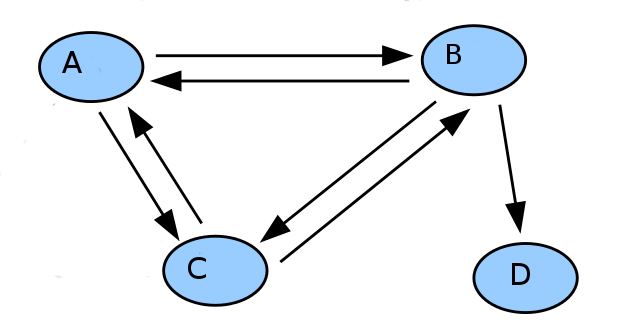
\includegraphics[width=8cm]{immagini/linkfarm/linkfarm}
\caption{Struttura di una link farm.}
\label{fig:linkfarm}
\end{figure}

\section{Link dai forum}
Un metodo utilizzato dagli spammer per creare delle grandi link farm è lo scambio di link che molto spesso avviene attraverso l'utilizzo di forum SEO (Search Engine Optimization). Questi forum contengono varie tipologie di discussioni  (ad esempio spiegazioni su come manipolare gli algoritmi dei motori di ricerca per incrementare il rank delle pagine e sezioni dedicate anche allo scambio dei link). Utilizzando tali informazioni si potrebbe costruire un algoritmo per identificare i siti spam e quindi azzerare o attenuare il loro valore di rilevanza delle ricerche in un motore di ricerca. Tale processo non è semplice in quanto la presenza di numerose e diversificate informazioni producono rumore nel rilevamento dei link. Un modo efficace per implementare questa tecnica consiste nel  \cite{Cheng:2011:LWS:1935826.1935902}: 
\begin{itemize}
 \item Estrarre tutti i link contenuti nei post.
 \item Dal momento che non tutti i link presenti nei post sono spam vengono estratte le feature dai link sulla base delle loro relazioni con gli utenti del forum e della struttura dei loro link nel grafo del web. Le feature vengono catalogate in tre tipi: feature del forum SEO (quali la frequenza di URL nel forum, il numero di thread che il proprietario dell'URL ha discusso, il numero di post autorizzati dal proprietario dell'URL, il numero di URL inseriti dal proprietario dell'URL, la media degli URL per post di un utente, il numero di post che contengono l'URL del proprietario), le feature del grafo (fra cui il numero di link in ingresso, il numero di link in uscita, la media dei link in uscita dei vicini in ingresso, la media dei link in entrata dei vicini in uscita) e le feature del sito (la lunghezza dell'URL). 
 \item Infine viene calcolato il valore di spam dei siti.
\end{itemize}
Questi metodi sono di particolare aiuto nell'incrementare il numero di pagine spam che i metodi convenzionali (sia basati sul contenuto che sulla struttura del grafo) non riescono a identificare  e perciò è possibile usarlo come metodo complementare ai metodi classici. 


\section{Metodi per migliorare la classificazione}
Oltre alla rilevazione delle pagine di spam utilizzando le tecniche e le feature descritte in precedenza, un aspetto focale consiste nel miglioramento della fase di classificazione; in \cite{Gan:2007:IWS:1244408.1244412} viene presentato un metodo per migliorare la classificazione  utilizzando un classificatore di base, per etichettare le pagine, e delle euristiche basate sulla tipologia dei nodi vicini a un nodo \(v\). Tali euristiche determinano se il nodo \(v\) dovrebbe essere rietichettato basandosi sul risultato della prima classificazione o sull'informazione tratta dalle euristiche. Gli autori di tale metodo affermano che  la struttura dei vicini di un nodo è un buon indicatore  per classificarlo in  spam o non spam. In particolare vengono analizzate alcune distribuzioni delle proprietà dei vicini:
\begin{itemize}
 \item la distribuzione dello spam in entrata: tale distribuzione è rappresentata  tramite il grafico in figura \ref{img:gan1}  dove ogni sito (di cui si conosce se esso è spam o non spam) andrà a finire in uno dei settori sull'asse \(x\) in base alla frazione di nodi spam tra i sui vicini in entrata. L'asse \(y\) rappresenta la percentuale di spam/non spam all'interno del settore. Dal grafico si nota che quanto più è alta la frazione di vicini spam in entrata di un sito tanto la probabilità che tale sito sia spam cresce.  
 \begin{figure}
 \centering
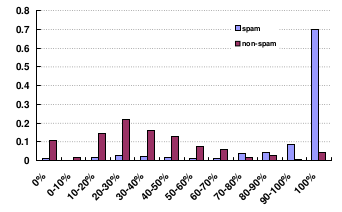
\includegraphics[width=10cm]{immagini/gan/immagine1.png}
\caption{Distribuzione dello spam in entrata}
\label{img:gan1}
\end{figure}
\item la distribuzione dello spam in uscita: tale distribuzione è rappresentata  tramite il grafico in figura \ref{img:gan2}; si osserva che tale distribuzione è simile a quella per lo spam in entrata.
 \begin{figure}
 \centering
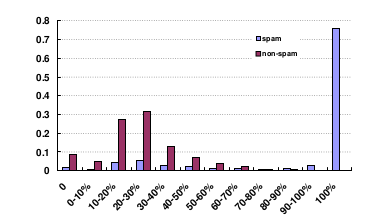
\includegraphics[width=10cm]{immagini/gan/immagine2.png}
\caption{Distribuzione dello spam in uscita}
\label{img:gan2}
\end{figure}
\item distribuzione entrante pesata: tale distribuzione è rappresentata  tramite il grafico in figura \ref{img:gan3}; in tale distribuzione vengono esaminati gli inlink pesati con pagerank.
 \begin{figure}
 \centering
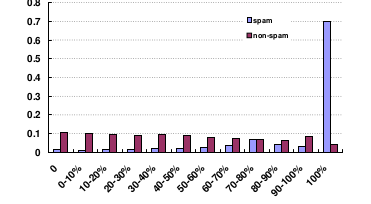
\includegraphics[width=10cm]{immagini/gan/immagine3.png}
\caption{Distribuzione entrante pesata}
\label{img:gan3}
\end{figure}
\end{itemize}
Vi sono due approcci per rietichettare i nodi dopo la prima classificazione. Nel primo, a ogni nodo viene assegnata un etichetta dal primo classificatore e successivamente viene definita un'altra etichetta per un nodo vicino, sulla base di una delle euristiche definite in precedenza, a cui viene associato un livello di confidenza; quindi l'etichetta del nodo determinata attraverso la classificazione di base viene confrontata con quella di un nodo vicino, se le due etichette sono molto difformi tra loro e l'etichetta del nodo vicino è molto affidabile in termini di confidenza allora l’etichetta del sito viene cambiata da spam a non spam (o viceversa). Il secondo modo consiste nel applicare, dopo la classificazione di base, un secondo classificatore che utilizza altre feature ( le etichette assegnate dal primo classificatore, la percentuale di inlink corrispondenti a siti spam, la percentuale di outlink che puntano a siti spam, ecc...).

Un altro metodo che fa uso della riassegnazione delle etichette associate a ogni nodo dopo una prima fase di classificazione è descritto in \cite{Geng:2008:IWS:1367497.1367685}. Tale metodo fa uso di una strategia di riestrazione delle feature facendo delle analisi basate sui clustering dei nodi, analisi sulla propagazione e analisi basate sulla struttura del grafo dei nodi vicini. L'algoritmo è suddiviso in quattro fasi:
\begin{itemize}
 \item vengono estratte delle feature base per ogni nodo;
 \item viene eseguita una prima classificazione;
 \item successivamente vengono riestratte le altre feature basate sui cluster, sulla propagazione e sulla struttura dei vicini;
 \item viene rieseguita una seconda fase di classificazione;
\end{itemize}
Le analisi sui cluster vengono eseguite utilizzando un grafo non diretto \(G=(V,E,w)\), dove \(V\) è l'insieme degli host, \(w\) è una funzione di pesatura e \(E\) è l'insieme degli archi con peso non zero. Quindi per calcolare la feature sui cluster il grafo viene partizionato in \(k\) cluster e successivamente calcolato:
\begin{equation}
 cf(H)=\frac{\sum_{h\in C(H)}spamicity(H)}{|C(H)|}
\end{equation}
dove \(C(H)\) è il cluster al quale l'host \(H\) appartiene e la \(spamicity(h)\) è il valore di spam rilevato durante la prima classificazione.\\
Diversamente la feature di propagazione si ottiene nel seguente modo:
\begin{equation}
 pf(H)^{(t)}=\sum_{h:h->H}\frac{pf(h)^{t-1}\times weight(h,H)}{\sum_{g:h->g}weight(h,g)}
\end{equation}
dove \(t\) è il numero di iterazioni, \(pf(h)^{(0)}=spamicity(h)\) e \(weigth(h,H)\) è il peso degli host \(h\) e \(H\).\\ 
Infine l'ultima feature quella relativa alla struttura dei vicini si ottiene:
\begin{equation}
 nf(H)=\frac{\sum_{h\in N(H)}(sapmicity(h)\times weight(H,h))}{|N(H)|}
\end{equation}
dove \(N(H) \in \{inlink(H), outlink(H), outlink(outlink(H)), inlink(inlink(H)),\\ inlink(outlink(H)), outlink(inlink(H))\}\) e quindi rappresenta l'insieme delle relazioni con i nodi vicini del nodo\ \(H\) .

Le prestazioni della fase di classificazione degli algoritmi di spam detection sono legate al quantità di dati di traning con cui il classificatore viene istruito.  le performance della classificazione, quindi, in \cite{Geng:2009:LBS:1526709.1526920} viene proposto un particolare algoritmo di apprendimento supervisionato denominato \textit{Link-training}; tale algoritmo si basa sull'apprendimento dai link ovvero la dipendenza topologica. L'algoritmo di apprendimento si può riassumere nei seguenti passi:
\begin{itemize}
 \item La prima fase consiste nel istruire un classificatore attraverso l'uso di un piccolo dataset.
 \item Successivamente viene utilizzato il classificatore per categorizzare e assegnare un valore di spam (\textit{PS}) ai dati non etichettati; il calcolo di \textit{PS} avviene nel seguente modo:
 \begin{equation}
  PS(x)=\frac{P_{spam}(x)}{P_{spam}(x)+P_{normal}(x)}
 \end{equation}
 dove, \(P_{spam}(x)\) è la probabilità di \(x\) di essere un nodo spam.
 \item Il passo successivo consiste nell'assegnare a tutti i nodi il valore di spam calcolato.
 \item Per istruire il classificatore oltre al valore di spam di base viene calcolato anche quello relativo ai vicini (LS):
 \begin{equation}
LS(h)=\frac{\sum_{v\in N(h)}(PS(v)\times weight(h,v))}{\sum_{v\in N(h)}weight(h,v)}
 \end{equation}
dove \(v\) e \(h\) sono gli host, \(weight(h,v)\) è il peso dell'host \(h\) e \(v\) , \(weight(h,v\in {1,\log{(n)}})\), dove \(n\) è il numero di link tra i due nodi. \(N(h)\in inlink(h) \cup outlink(h)\), dove \(inlink(h)\) rappresenta l'insieme dei link in entrata di \(h\) e \(outlink(h)\) rappresenta l'insieme dei link in uscita di \(h\). 
Queste fasi del processo sono cicliche per un numero stabilito di iterazioni.
\end{itemize}

Gli algoritmi di spam detection basati sul grafo ottenuto dalla fase di crawling sfruttano le caratteristiche dei grafi per ottenere delle informazioni riguardo i nodi spam. Quasi tutti i metodi descritti si basano sulla stessa intuizione dell'algoritmo di \textit{trustrank} (quella relativa all'isolazione approssimata delle pagine buone) sfruttando tale intuizione per determinare le pagine spam. Ad esempio \textit{Anti-trust rank} sfrutta tale intuizione ma non andando a manipolare i link in uscita di ogni nodo ma i link dei nodi entranti. Altri metodi mentre si basano sulla ricerca delle spam farm mentre altri ancora si focalizzano sul miglioramento dei vari algoritmi di classificazione. Oltre alle tecniche basate su contenuto e sul grafo del web sono state implementate altre che utilizzano criteri diversi per determinare le pagine spam che non si possono identificare tramite i metodi classici; tali metodi, quindi, sono nati per andare incontro alla crescita di nuovi tipi di web spam.




